\documentclass[journal]{vgtc}               
\ifpdf%                                % if we use pdflatex
  \pdfoutput=1\relax                   % create PDFs from pdfLaTeX
  \pdfcompresslevel=9                  % PDF Compression
  \pdfoptionpdfminorversion=7          % create PDF 1.7
  \ExecuteOptions{pdftex}
  \usepackage{graphicx}                % allow us to embed graphics files
  \usepackage[section]{placeins}
  \DeclareGraphicsExtensions{.pdf,.png,.jpg,.jpeg} % for pdflatex we expect .pdf, .png, or .jpg files
\else%                                 % else we use pure latex
  \ExecuteOptions{dvips}
  \usepackage{graphicx}                % allow us to embed graphics files
  \DeclareGraphicsExtensions{.eps}     % for pure latex we expect eps files
\fi%

%% it is recomended to use ``\autoref{sec:bla}'' instead of ``Fig.~\ref{sec:bla}''
\graphicspath{{figures/}{pictures/}{images/}{./}} % where to search for the images

\usepackage{microtype}                 % use micro-typography (slightly more compact, better to read)
\PassOptionsToPackage{warn}{textcomp}  % to address font issues with \textrightarrow
\usepackage{textcomp}                  % use better special symbols
\usepackage{mathptmx}                  % use matching math font
\usepackage{times}                     % we use Times as the main font
\renewcommand*\ttdefault{txtt}         % a nicer typewriter font
\usepackage{cite}                      % needed to automatically sort the references
\usepackage{tabu}                      % only used for the table example
\usepackage{booktabs}                  % only used for the table example
%% OnlineID. Otherwise, you may safely leave it at ``0''.
\onlineid{0}

\vgtccategory{Research}
\vgtcpapertype{theory/model}

\newpage
%% Paper title.
\title{CS 458 - OSU Course Planner}

%% This is how authors are specified in the journal style

%% indicate IEEE Member or Student Member in form indicated below
\author{Miles McCall, Shane Barrantes}
\authorfooter{
%% insert punctuation at end of each item
\item
 Miles McCall E-mail: mccallm@oregonstate.edu
\item
 Shane Barrantes E-mail: barrants@oregonstate.edu
}

%% Abstract section.
\abstract{
	This document describes the visualization problem we chose for our midterm project. It addresses our design process for a new solution, including our goals, user interface philosophies, research on related projects, and the result of our prototype implementation. 
} % end of abstract

%% Keywords that describe your work. Will show as 'Index Terms' in journal
%% please capitalize first letter and insert punctuation after last keyword
\keywords{OSU, MyDegrees, Planner, Scheduler, Courses, Visualization}

%% Uncomment below to include a teaser figure.
\teaser{
	\frame{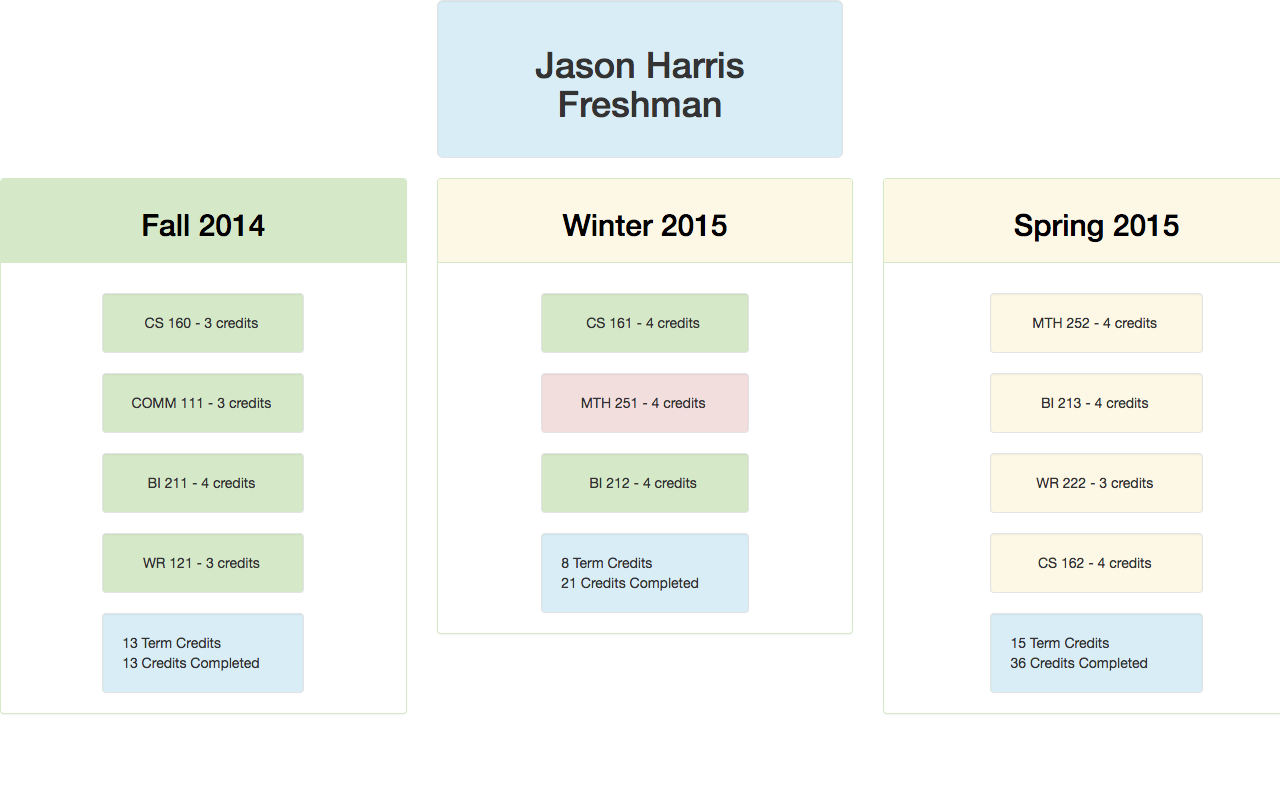
\includegraphics[width=\linewidth]{pictures/final_CS458.png}}
   	\caption{Year View}
	\label{fig:teaser}   
}

%%%%%%%%%%%%%%%%%%%%%%%%%%%%%%%%%%%%%%%%%%%%%%%%%%%%%%%%%%%%%%%%
%%%%%%%%%%%%%%%%%%%%%% START OF THE PAPER %%%%%%%%%%%%%%%%%%%%%%
%%%%%%%%%%%%%%%%%%%%%%%%%%%%%%%%%%%%%%%%%%%%%%%%%%%%%%%%%%%%%%%%%

\begin{document}
\maketitle
\tableofcontents

\section{Introduction}
The current academic self monitoring system used at Oregon State University, also known as MyDegrees, provides a wealth of information about any particular student, however this information is obfuscated behind poor layout, color scheme, and overall visual design. This lack of presentableness and usability hinders students and advisors alike when trying to understand a student's current standing including classes they have completed for college credit, classes they still need to take, and their overall path to graduation. In an attempt to make this path to graduation more clear we created a new modularized system of visualization that allows students to easily view detailed class information as well as what classes they need to complete each term and year while they attend Oregon State University. This system uses typical color coding schemes to make it abundantly clear to our users which classes have been successfully passed, which still need to be taken, and which need to be retaken to achieve college credit.

\subsection{Visualization tasks}
  \begin{itemize}
    \item Clearly organize class data in modulus so that users can envision a clear scheduling path to graduation by term, year, and all years. 
    \item Add color coding scheme to add ease of visibility to the current state of classes (i.e. credit achieved, credit not achieved, currently in progress)
    \item Apply Gestalt Principles of proximity and similarity to group classes, terms, and years together.
   \end{itemize}
   
\section{Related Works}
Looking for related works which achieve an easily visualized system for detailed schedules is quite difficult because college schedules are incredibly complicated with different schools having different majors and paths to graduation. This is exacerbated by the fact that we do not have access to other colleges' course planning tools. However, because our goals are simply to make visualization easier and MyDegrees already has several visualization tools it sufficiently fulfills the requirement as a related work. In comparison to our visualization the information is far less logically laid out in a visually pleasing way and does not utilize a color coding system which obfuscates the data. 

The other class scheduling technologies we were able to find online consist of primarily a week by week view with no integration with college catalogs. While these tools are useful, they don't assist a more broad perspective on taking classes and generally don't implement color or make significant use of gestalt principles.

\section{Methods}
The tools and libraries we used for our course planner consist of the programming language PHP, the relational database system MySQL, and the front libraries known as the framework Bootstrap. We chose to use PHP because we did development on OSU's server and we know that an up to date version existed for our needs. We chose to use MySQL over other database management tools since it is the most widely used and doesn't include as much overhead as other comparable management tools like PostGreSQL. Finally, we chose to use Bootstrap for our front end because it suited our purpose extremely well and is widely used in the industry.

The actual implementation of our Course Planner uses MySQL to store course information in a database. We only included a small subset of data for rendering purposes, however if we were to fully create this product we would need the database to store the entirety of Oregon State's course catalog in a logical way. We then use PHP to access the database information and programmatically build our front end based on the data gathered from the database. Finally, that front end consists of Bootstrap's custom CSS and pre-built HTML components.

\section{Results}
In this section we will discuss the results of our fully visualised Oregon State University course planner. 

\begin{center}
	\frame{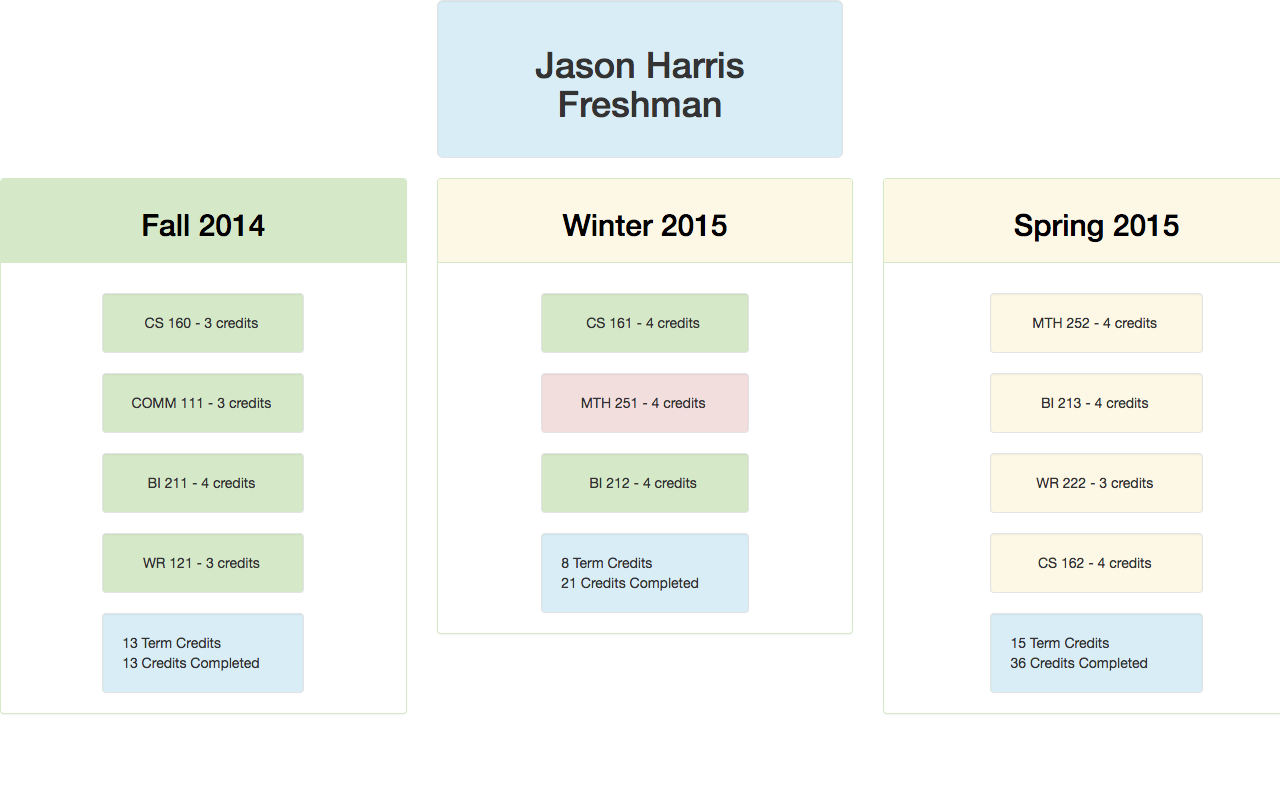
\includegraphics[width=\linewidth]{pictures/final_CS458.png}}
\end{center}

As you can see above the created course catalog pulls the student name and 
year to populate the header. It then populates three term sections with information that corresponds directly the students long term schedule. Finally, it changes the color of the class boxes depending on the student's status of the course. For example, a green box means that the course has been completed successfully, a yellow course means that the student is currently taking that course, and a red box means that the student failed a course and needs to retake it for college credit.

\section{Conclusion}
Our visualization project proceeded with the goal to provide Oregon State University students with a much needed tool to better visualize their path to collegiate graduation. To do this, we implemented a color coded system, a year at a glance perspective, and gestalt principles of grouping to make a visually pleasing and useful design. 

The most difficult part of this project was to design a method for storing so much information in such a confined place while still making it logically and visually pleasing. To do this we designed a modular system, unfortunately due to time constraints and the large scope of our project we were only able to render the year at a glance submodule. In order to improve our project we would have liked to fully fledge out every page that we discussed in our initial document as well as populate our database with the entire Oregon State course catalog.

By simplifying and automating students' course schedules, our visual model can solve more than just one student's problems. The university itself could adopt this tool as an administration tool. If the course planning tool was scaled to incorporate all enrolled students, the system's algorithm could generate schedules that minimize wait-listing while still providing individual students with flexibility in their schedules. The algorithm would dynamically update based on user inputted preferences and restrictions, and references the entire OSU course catalog to provide useful data. 

During registration periods for each new term, the school's servers are notorious for under-performing under load which directly affects students' lives. It may seem like a negligible issue, but with the limited availability of certain courses a student could be delayed for graduation simply because they couldn't register properly online. With our algorithm generating schedules for all users ahead of time, the load on the network would be greatly reduced during these periods. This solution also saves the administration and registration offices a great deal of work resolving issues with registration. Unless there are major issues or conflicts for a particular student, only a simple confirmation of the generated schedule is needed from each user. 

\section{Named Contributions}
  \begin{table}[!h]
    \centering
    \caption{Task Distribution}
    \begin{tabular}{|l|cc|}
      \hline
      \textbf{Project Task}    & \textbf{Miles} & \textbf{Shane} \\ \hline
      software tool selection  & X              & X              \\
      front-end design         & X              & X              \\
      front-end implementation &                & X              \\
      database design          & X              & X              \\
      database implementation  & X              &                \\
      written report           &                & X              \\
      query design             & X              & X              \\
      query implementation     & X              &                \\ \hline
    \end{tabular}
  \end{table}

\end{document}

